%!TEX root=../document.tex

\section{Angabe}
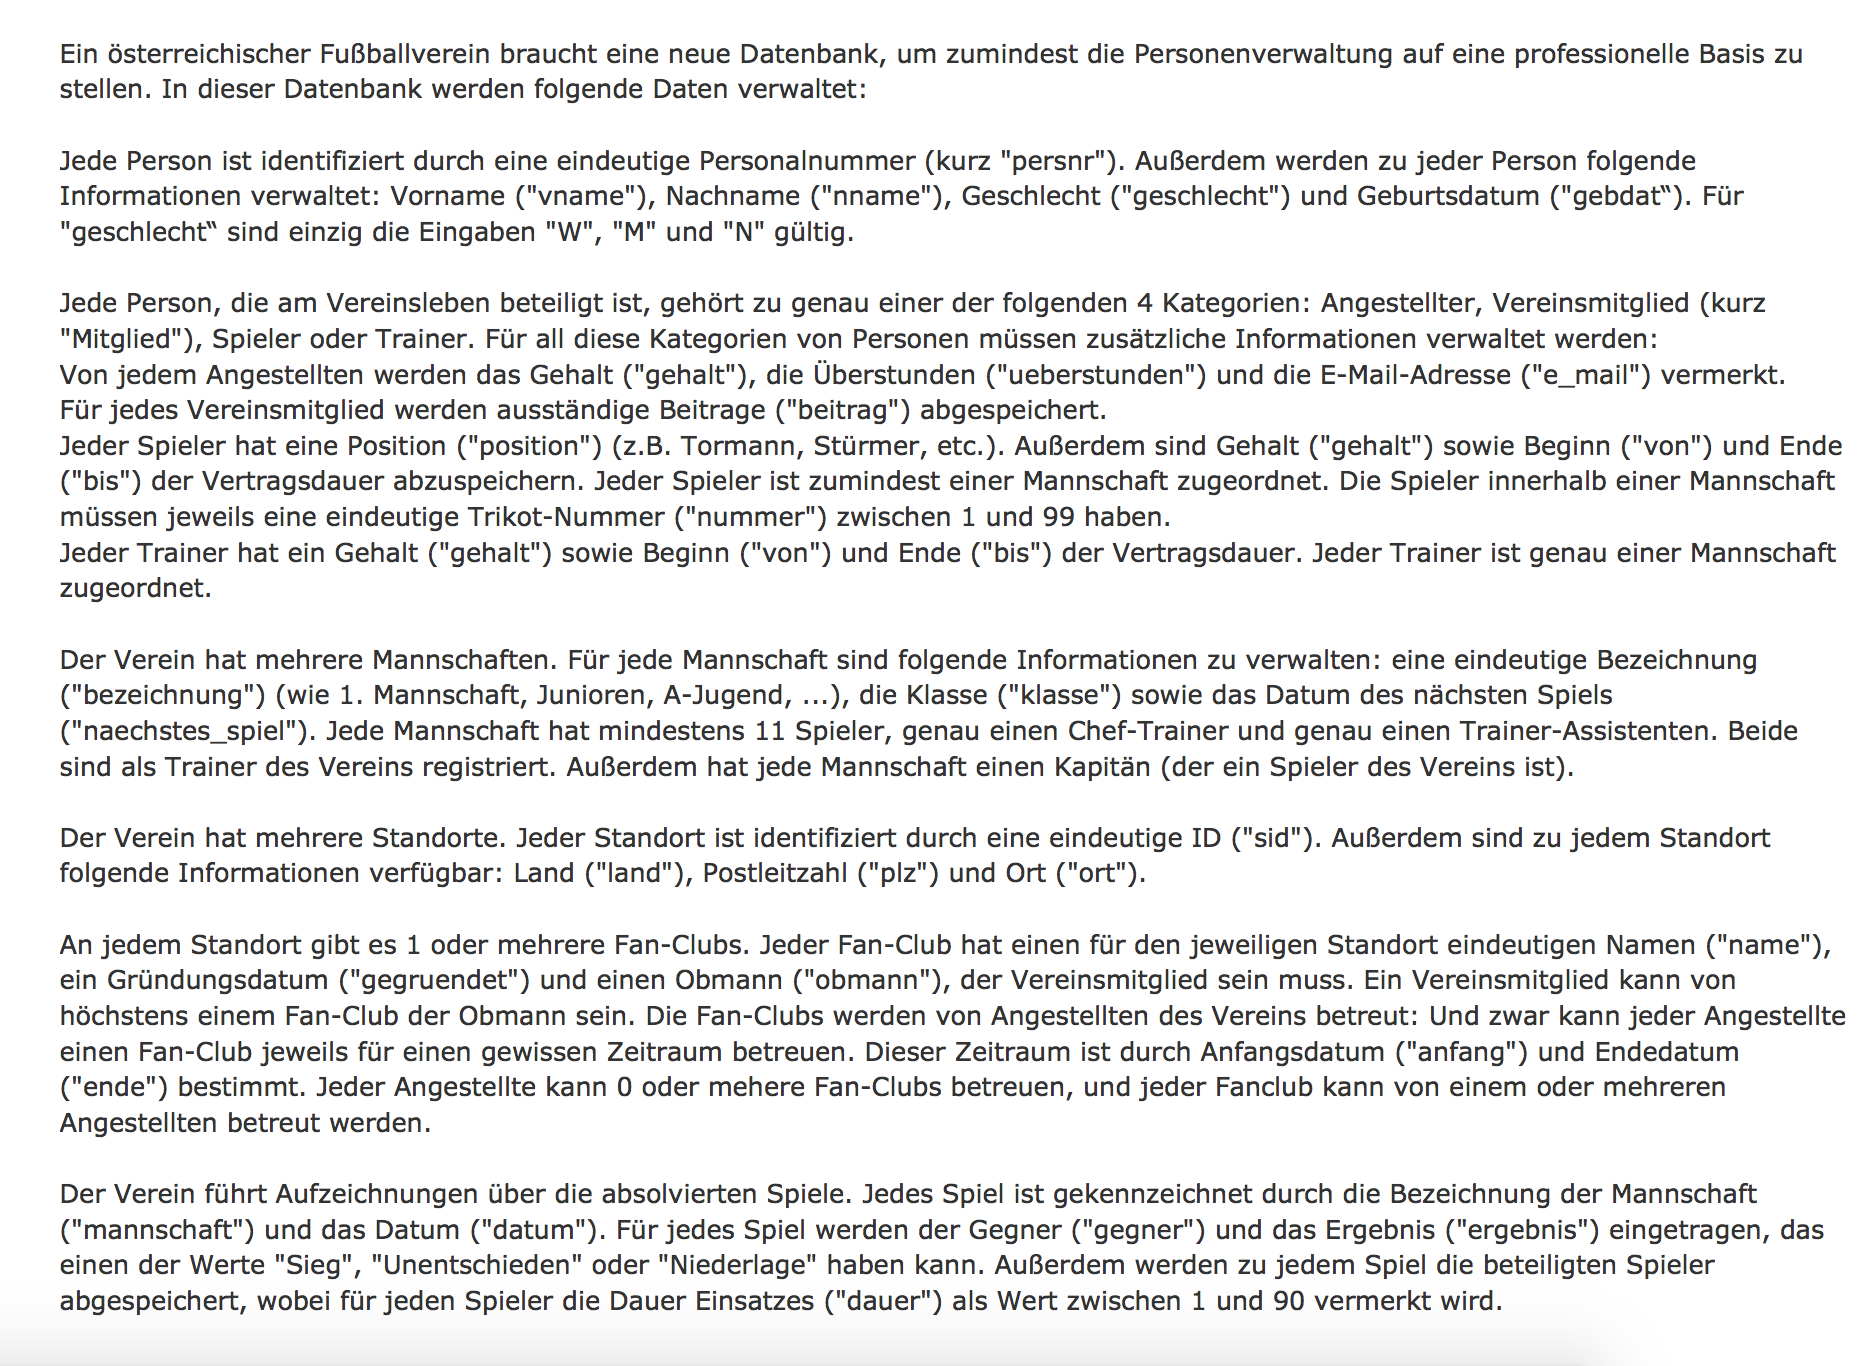
\includegraphics[scale=0.5]{images/angabe.png}

\section{Vorraussetzungen}
\subsection{Server starten}
\subsection{SSH - Verbindung}
\subsection{Postgres}
Datenbank, User erzeugen, Rechte verteilen \& Einloggen

\begin{lstlisting}
CREATE DATABASE verein;
CREATE USER manager WITH PASSWORD 'iderfrein';
GRANT ALL ON DATABASE verein TO manager;
\end{lstlisting}

Connection :
\begin{lstlisting}
psql -d verein -h localhost -U manager
\end{lstlisting}
\section{Aufgaben}

\subsection{CREATE-Befehle}
Schreiben Sie die n�tigen CREATE-Befehle, um die vorgestellten Relationen mittels SQL zu realisieren.
Dabei sind folgende Punkte zu beachten:

\subsubsection{Die Datenbank soll keine NULL-Werte enthalten.}
Dies l�sst sich umsetzen, indem man am Ende des Attributes ein 'NOT NULL' anf�gt.\newline
Beispiel:
\lstinputlisting[language=SQL, firstline=16, lastline=22]{../../sql/create.sql}

\subsubsection{Realisieren Sie folgende Attribute mit fortlaufenden Nummern...}
...mit Hilfe von Sequences und Serial: "persnr" von Personen und ''sid'' von Standorten.
\begin{itemize}
\item F�r das ''persnr'' - Attribut sollen nur gerade, 5-stellige Zahlen vergeben werden (d.h.: 10000, 10002, ..., 99998).\newline

Sequences kann man sich wie eine Z�hlervariable vorstellen, welche im Hintergrund mitl�uft.
Erstellt wird unsere Sequence so :
\lstinputlisting[language=SQL, firstline=5, lastline=5]{../../sql/create.sql}

Die 5 Stellen erhalten wir, indem wir uns an der Option \textbf{START WITH} bedienen.\newline
F�r die geraden Zahlen helfen wir uns mit einem Trick, in dem wir mit Hilfe von \textbf{INCREMET BY} immer um 2 erh�hen.\newline
=> da er nur immer um 2 erh�ht, k�nnen nur gerade Zahlen kommen ! \newline

\item F�r das ''sid'' - Attribut sollen beliebige positive Zahlen (d.h. 1,2, ...) vergeben werden.\newline
Falls zwischen 2 Tabellen zyklische FOREIGN KEY Beziehungen herrschen,
dann sind diese FOREIGN KEYs auf eine Weise zu definieren, dass es m�glich ist, immer weitere Datens�tze mittels INSERT in diese Tabellen einzuf�gen.\newline
Die positiven Zahlen erhalten wir mittels einer \textbf{CHECK} - Constraint.\newline
\lstinputlisting[language=SQL, firstline=68, lastline=68]{../../sql/create.sql}

\end{itemize}

\subsection{INSERT-Befehle}
Schreiben Sie INSERT-Befehle, um Testdaten f�r die kreierten Tabellen einzurichten. \newline
Jede Tabelle soll zumindest 10.0000 Zeilen enthalten. \newline
Sie d�rfen die Wahl der Namen, Bezeichnungen, etc. so einfach wie m�glich gestalten, d.h.: Sie m�ssen nicht "real existierende" Fu�baller-Namen, L�nder, St�dte, etc. w�hlen. \newline
Stattdessen k�nnen Sie ruhig 'Spieler 1', 'Spieler 2', 'Land 1', 'Land 2', 'Stadt 1', 'Stadt 2', etc. verwenden. \newline
Sie k�nnen f�r die Erstellung der Testdaten auch entsprechende Generatoren verwenden! \newline


\subsection{DROP-Befehle}
Schreiben Sie die n�tigen DROP-Befehle, um alle kreierten Datenbankobjekte wieder zu l�schen.
z.B
\lstinputlisting[language=SQL, firstline=2, lastline=2]{../../sql/drop.sql}

\section{Probleml�sungen mittels SQL}
\subsection{Fanclub-Betreuung}
W�hlen Sie "per Hand" die Personalnummer eines Angestellten aus Ihren Testdaten aus.\newline
Schreiben Sie eine SQL-Anfrage, die jene Fan-Clubs ermittelt, die dieser Angestellte im Moment nicht betreut.\newline
Geben Sie zu jedem derartigen Fan-Club die Standort-ID und den Namen des Fan-Clubs aus.\newline
Bemerkung: Ein Fan-Club wird von einem Angestellten im Moment nicht betreut,\newline
wenn entweder der Angestellte diesen Fan-Club �berhaupt nie betreut hat\newline
oder wenn das heutige Datum (= sysdate) au�erhalb des Betreuungszeitraums liegt.\newline
Vergessen Sie nicht, jene Fan-Clubs zu ber�cksichtigen,\newline
die von �berhaupt keinem Angestellten betreut werden (dieser Fall sollte zwar laut Datenmodell nicht vorkommen.\newline
Die Einhaltung dieser Bedingung wird aber vermutlich vom Datenbanksystem nicht �berpr�ft)!\newline
